\section{The old DAC Systems}

In this section, I shall summarize the works done previously by Zero Emission Fuels B.V relating to the Direct Air Capture System (DAC). Before starting my work at the internship in the ZEF V team. I have to read and learn what was already worked on by the previous interns and thesis students. So that, I can get an idea in-order to know what has been done, what works and to know what can be done further. The section with be divided into various subsections starting from ZEF I to ZEF IV. In each of the subsections, the work done by them and their findings shall be elaborated further. 

\subsection{ZEF I - the beginning}

According to the internship report submitted by Sjors and Sotiris \cite{Wagenaar2018}. The first DAC team realized that going about physical swing adsorption won't be feasible due to the low concentration of $CO_2$ in the atmosphere and flue gases is only about 10 - 15\% of the exhaust gases and moisture inhibits the kinetics for physical adsorbent. They also defined what are the characteristics required to be full-filled in finding the candidate adsorbent which was having :-

\begin{itemize}
    \item High adsorption capacity
    \item High kinetics 
    \item Chemical and Thermal stability
    \item Low cost 
    \item Fouling resistance 
    \item No promotion of unwanted by-products
\end{itemize}

On further literature study, it was determined that most accepted study is the Impregnation of Polyethylenemeine (PEI) on mesoporous silica. It was also determined that the adsorbent must be heated to 120 \degree C  in-order to desorb the $CO_2$. \textbf{Note:} It is critical to note that PEI in combination with $O_2$ at high temperatures (around 120 \degree C) causes sorbent degradation. 

\subsubsection{Design}
The input feedstock for the ZEF plant is 187 grams of $CO_2$ in 8 batches (batch process). A container of 3L capacity was 3D printed using PLA material and various kinetics studies were conducted to determine the adsorption and desorption characteristics of PEI. The DAC column is chosen to be a packed bed reactor as there seems to be a lot of design issues with multiple layer fluidized bed system. The reactor bed was 3D printed using Polycarbonate (PC) material as it is the only material that can withstand the sorbent heating to 120 \degree C for desorption. The absorption and desorption of $CO_2$ is going to be taking place simultaneously in 2 seperate chambers which can be seen more elaborately in Figure \ref{fig:zef1ads} and Figure \ref{fig:zef1des} and in Figure \ref{fig:zef1ass} we can see the isometric view of the DAC unit that was designed and fabricated by the ZEF I team. 

\begin{figure}[H]
\centering
\begin{minipage}{.5\textwidth}
  \centering
  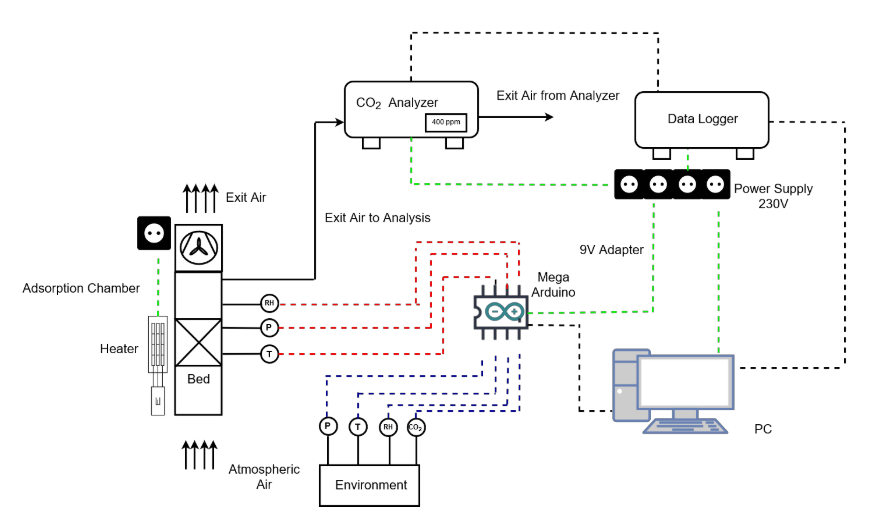
\includegraphics[width=\linewidth]{images/previouswork/zef1ads.png}
  \captionof{figure}{Schema of adsorption process \cite{Wagenaar2018}}
  \label{fig:zef1ads}
\end{minipage}%
\begin{minipage}{.5\textwidth}
  \centering
  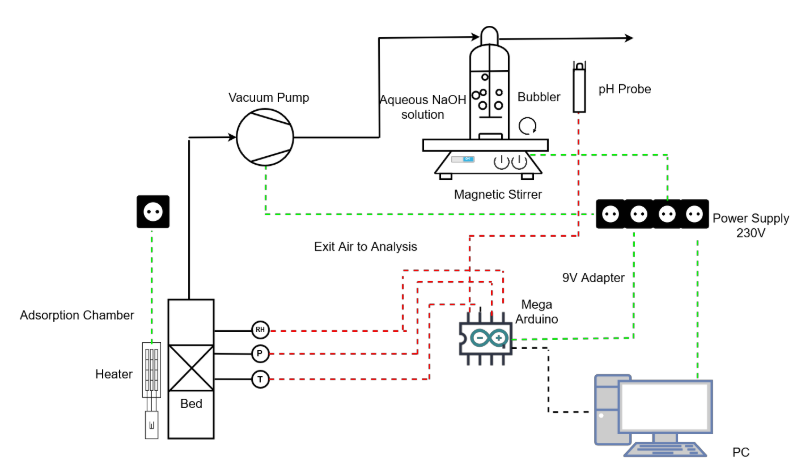
\includegraphics[width=\linewidth]{images/previouswork/zef1des.png}
  \captionof{figure}{Schema of desportion process \cite{Wagenaar2018}}
  \label{fig:zef1des}
\end{minipage}
\end{figure}

\begin{figure}[H]
    \centering
    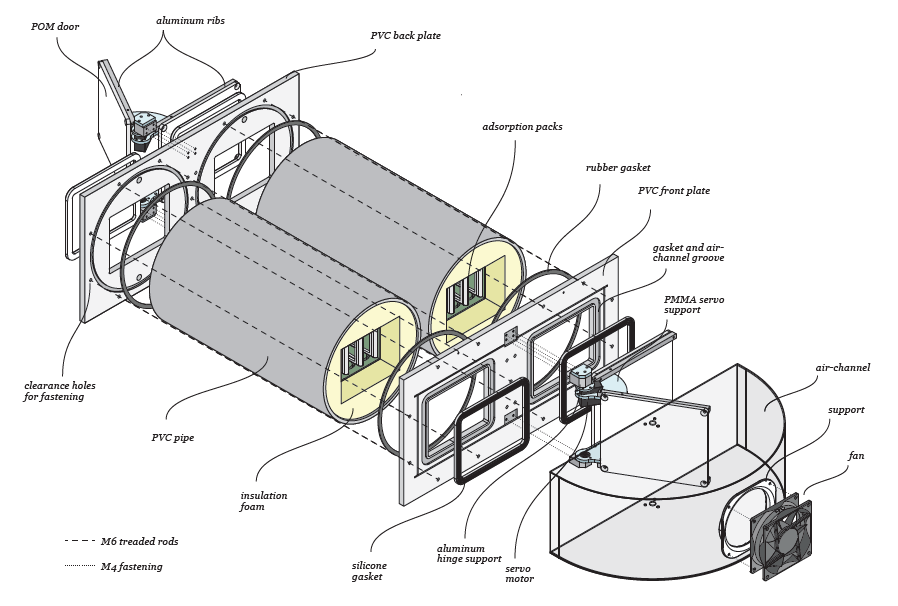
\includegraphics[width=\linewidth]{images/previouswork/zef1ass.png}
    \caption{Isometric view of the DAC unit assembly \cite{Azzalini2018}}
    \label{fig:zef1ass}
\end{figure}

\subsubsection{Further work}
The DAC team of ZEF 1 got a DAC system running from scratch. However, the heating and cooling systems were not installed. Hence, no system testing could be performed. Some of the relevant conclusions and recommendations put forward by the team was :

\begin{itemize}
    \item In order to address the fluctuations in sensor readings. Powering the sensors using a stable and constant 9V power adapter is required. 
    \item Selection of a cheaper sorbent material such as amine grafter sugarcane bagasse. 
    \item Since PEI is a non - newtonian fluid, higher $CO_2$ absorption might be observed in order to optimize the parameter. 
    \item Innovative designs might help in better heat utilization for the other sub-systems and can aid in the adsorption of $CO_2$ in DAC. 
    \item Testing with the heating and condensation units must be carried out. 
\end{itemize}

\subsection{ZEF II - the shift to monoliths}




\subsection{ZEF III - }



\subsection{ZEF IV - }
\label{sec:zef4}














